\subsection{Extraction des composantes de l'intrant et des sources d'information à analyser}
Une fois que la requête de l'utilisateur aura été convertie sous une forme textuelle facilement manipulable par un ordinateur, nous pourrions, dès lors, utiliser le plongement induit par l'étape précédente. Une autre approche consiste à reprendre cette sortie pour ensuite la fournir à une nouvelle structure qui se chargera d'aller extraire de nouvelles composantes qui aideront certainement à obtenir de meilleurs résultats pour la suite du processus. \\

À ce stade, nous devons comprendre que le signal est encore purement textuel et nous n'avons pour seule information qu'une décomposition des mots qui forment la demande reçue. Cependant, les langages sont formés de davantage de subtilités qu'un simple enchaînement de mots les uns après les autres. En effet, chaque mot joue un rôle précis dans la structure de la phrase et apporte une nuance particulière au contexte générale de celle-ci ou encore du texte avec une plus faible portée. C'est exactement ce que les travaux de ... visaient à faire. Ainsi, en ..., ce groupe de chercheurs a fait la publication d'un article détaillant leur approche en comparant plusieurs modèles différents comprenant autant des approches classiques que des approches neuronales. En plus de faire état de leurs travaux, ce groupe est aussi à l'origine d'outil qui est encore à ce jour considéré comme un incontournable: \cite{word2vec}. \\

Malgré le fait que cet article porte sur les approches neuronales, cet outil a plutôt prouvé que des approches plus simplistes et classiques sont parfois plus appropriées. Word2vec se fonde sur la combinaison de deux approches nommées \textit{Continuous Bag Of Words} (\autoref{fig:cbow}) et \textit{Skip-gram} (\autoref{fig:skipgram}). Alors que le \textit{Skip-gram} se concentre à essayer de prédire son contexte, le \textit{CBOW} cherchera plutôt à prédire la valeur considérée à partir de son environnement accordant ainsi plus d’importance à la structure des phrases plutôt qu’au contexte d’utilisation.\\

\begin{figure}[ht]
  \centering
  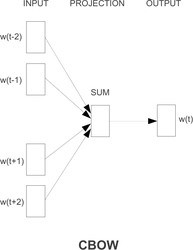
\includegraphics[width=\columnwidth, height=0.35\textheight, keepaspectratio]{cbow}
  \caption{Architecture de la méthode de prédiction CBOW [\citenum{word2vec}]}
  \label{fig:cbow}
\end{figure}

\begin{figure}[ht]
  \centering
  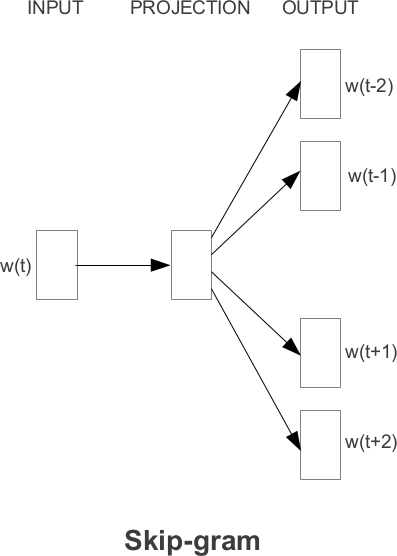
\includegraphics[width=\columnwidth, height=0.35\textheight, keepaspectratio]{skipgram}
  \caption{Architecture de la méthode de prédiction Skip-gram [\citenum{word2vec}]}
  \label{fig:skipgram}
\end{figure}

En fournissant la requête reçue à cet outil, il sera donc possible d'extraire les composantes sémantiques et syntaxiques sous-entendues par cette dernière. Par la suite, ces nouvelles composantes seront combinées à celle que nous avions déjà obtenues à l'étape précédente. En procédant avec cette seconde approche, nous réaliserons certainement un gain majeur au niveau de la performance des prochaines étapes en raison de l'ajout important de dimensionnalités qui fourniront beaucoup plus de flexibilité aux réseaux de neurones suivantes qui devront à leur tour détecter les nuances du langage. À titre d'exemple, lorsqu'un utilisateur demandera à l'assistant si ce dernier peut lui indiquer l'horaire du cinéma le plus prêt de sa position, l'assistant devra comprendre la nuance que ce qui intéresse vraiment l'utilisateur est l'horaire et non pas l'évaluation booléenne de sa capacité à s'acquitter de cette tâche. Par contre, dans le cas où l'utilisateur demanderait à l'assistant si ce dernier peut le connecté à l'Internet, l'assistant devra dans ce cas faire l'évaluation de sa capacité et répondre en par affirmation à notre cher utilisateur. \\
%TODO Référence au transfer learning

Mais qu'en est-il de nos sources d'informations? En fait, le processus entier bénéficiera certainement qu'un travail similaire soit fait à ce niveau aussi. Pour ce faire, deux approches s'offrent encore à nous. La première consistant encore une fois à utiliser word2vec et la seconde repose sur le même principe, mais à un niveau supérieur d'abstraction en considérant cette fois l'utilité de chacune des phrases dans le texte plutôt que de se concentrer sur le rôle de chaque mot dans chaque phrase \cite{inferSent}. \\

En somme, toutes ces composantes ainsi dérivée pourrons ensuite être fournies en entrée d'un réseau de neurones tel qu'un RNN tel qu'il sera expliqué à section suivante.
